%
% background.tex
%
% Copyright (C) 2018 by Andre Martins Pio de Mattos <andrempmattos@gmail.com>.
%
% Internship Report
%
% This work is licensed under the Creative Commons Attribution-ShareAlike 4.0
% International License. To view a copy of this license,
% visit http://creativecommons.org/licenses/by-sa/4.0/.
%

%
% \brief Title page.
%
% \author Andre Martins Pio de Mattos <andrempmattos@gmail.com>
%
% \version 0.1.0
%
% \date 08/09/2019
%

\newpage

\section{Background} \label{sec:background}

%--------------------------------------------------------------------------------

\subsection{CubeSat Standard}

This work proposes a scientific experiment payload for CubeSats \cite{cubesat_101}, a nanosatellite \cite{small_spacecraft_state_of_art} standard. This standard of satellites consists of specific criteria for its shape, size, and weight, which help reduce costs due to the higher feasibility for mass-production and availability of off-the-shelf parts. Besides these benefits, the standardization reduces the development time and ease the access of transportation and deployment into space.

Essentially, CubeSats are satellites composed by small cube units, which might be combined to form larger spacecrafts and to attend the mission requirements and goals. This "unit" is referred to as a 1U, then a 1U CubeSat is a 10 cm cube with a mass of approximately 1 to 1.33 kg. \autoref{fig:exploded_view} shows an illustrative diagram of the internal architecture of a 2U CubeSat, containing the core modules (power management, data handling and communication), payloads\footnote{The "Radiation Monitor" illustrated in the diagram is the payload proposed in this work. It also presents its preliminary location inside the satellite} (primary and secondary experiments), solar panels, antennas and others auxiliary modules.

\begin{figure}[!ht]
    \begin{center}
        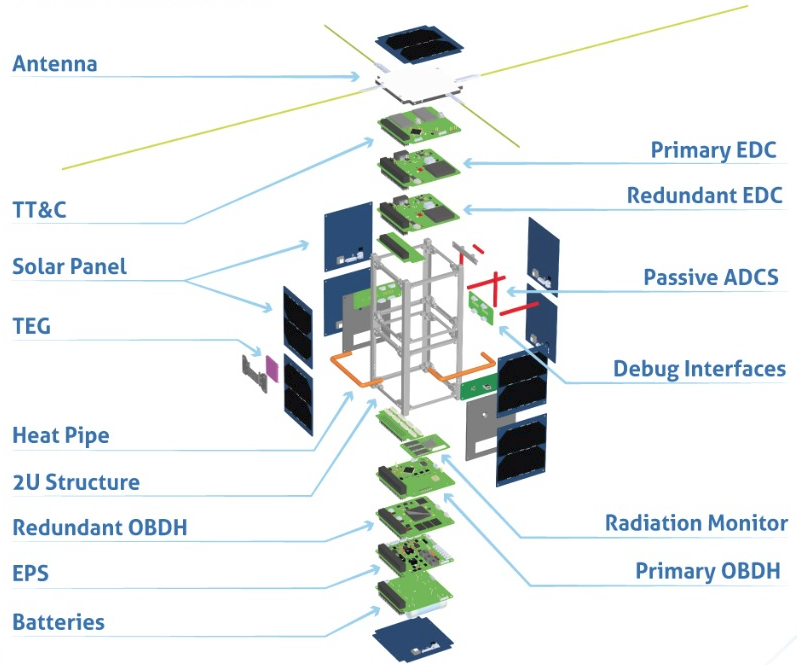
\includegraphics[width=0.85\textwidth]{figures/exploded_view.png}
        \caption{Conceptual exploded view of a CubeSat (GOLDS-UFSC).}
        \label{fig:exploded_view}
    \end{center}
\end{figure}

%--------------------------------------------------------------------------------

\subsection{Radiation Effects}

The space is full of engineering challenges related to the harsh environment conditions, including: mechanical stress, high temperature variations and severe radiation doses. This work focus on the last aspect, analysing its influence in electronic devices and evaluating the temporary and cumulative damaging phenomena. These effects are characterized by the Single Event Effects (SEEs), temporary, and the Total Ionizing Dose (TID) and Displacement Damage (DD), cumulative. The sensitive circuit nodes are affected or permanently damaged with the penetration of ionizing particles, which are representative outside the Earth's magnetic field protection.

The interaction with ionizing particles can induce the occurrence of instantaneous damaging events, which are characterized by the single event effects in various categories depending on the errors produced and the device components affected: Single-bit Upset (SBU), soft-error; Multiple-Bit Upset (MBU), soft-error; Multiple-Cell Upset (MCU), soft-error; Single Event Transient (SET), soft-error; Single Event Functional Interruption (SEFI), soft-error; Single Event Latch-up (SEL), hard/soft-error; Single Event Gate Rupture (SEGR), hard-error; and Single Event Burnout (SEB), hard-error. These effects might lead to soft-errors, errors that are reversible since can be mitigated by power cycles, resets, or other erase operations. In other cases, the effects induce hard-errors, leading to permanent device failure.

Both SBUs and MBUs are transient events that causes bit-flips (upsets) within a memory cell or latch, differing in the quantity of elements affected. Similarly, the MCUs are caused by the generation of two or more bit-flips within a cell array. The SETs are characterized by the collection of free carriers generated that induce a current or voltage transient that may lead to an error. The SEFIs are due to a perturbation in control signals, causing a loss of functionality and entering in a undefined state, a test mode, or a halt. The SELs occurs when a parasitic thyristor is triggered in the device structure, which generates high-current consumption and may lead to a thermal overheat in the affected region. The SEGRs occurs when a particle hit breaks the gate dielectric of a MOS transistor and the SEBs when a strike causes a destructive burnout due to high-currents.

The cumulative effects depends on the continuous exposure to radiation conditions that degrades the function of the device until its operation is definitely compromised. The TID is a long-term failure mechanism that causes shift in the transistors threshold voltage, increase of leakage currents (power consumption), and also the degradation of the gain in bipolar devices. The DD effect is the result of collisions between high-energy protons and the device that, when a minimum required energy is achieved, creates deformities in the lattice by removing the hit atom which results in different local electrical characteristics. The accumulation of this effect with energy above the displacement threshold can create a large fault cluster. For instance, it causes the reduction in bipolar transistor gain, reduction of the efficiency in solar cells, light emitting diodes and photodetectors, charge transfer inefficiency in charge coupled devices and resolution degradation in solid-state detectors.

%--------------------------------------------------------------------------------

\subsection{SDRAM Memories}

Synchronous dynamic random-access memories (SDRAM) are dynamic random-access memories (DRAM) whose operation is coordinated by an external supplied clock signal. The DRAM devices are a type of random access semiconductor memory that stores each bit of data in a cell structure based on a capacitor and a transistor. The capacitor retains or releases the energy during charge and discharge events controlled through the transistor. These two states, charged and discharged, represent the two values of a bit. However, due to parasitic coupling loads, the capacitor slowly leaks off, which leads to data loss after a certain period. Then, to prevent this, the device requires an external controller to perform periodic refresh cycles that rewrites the data in the capacitors, restoring them to their original initial charge.

The DRAM memories have the disadvantage of direct influence of input signals in the internal functions since each combination of control signals determine the execution of one memory operation (e.g, read, write, and refresh). Using a synchronous interface, it is possible to use pipeline techniques that improve the memory performance in comparison with asynchronous interfaces at the same frequency of operation. Pipelining means that the device can handle new commands before the termination a previous operation processing. Then, write and read commands can be followed by other commands after a fixed number of clock cycles (latency). Also, to improve even more the access operation speed, the memory is divided into equally sized sections called banks, which allows independent operations occurring simultaneously. This architecture enables SDRAMs to achieve greater concurrency and higher data throughput than the asynchronous memories.

These devices are susceptible to harsh radiation environments and many studies are carried out to evaluate their behavior in different conditions using ground-based experiments \cite{memory_tests_lucas}. This work, besides proposing a comparative study between different SDRAM chip generations, creates an experiment payload for in-orbit tests that might improve the ground-based evaluation methodology depending on the acquired results.

%--------------------------------------------------------------------------------

\subsection{FPGA Devices}

A Field-Programmable Gate Array (FPGA) is an integrated circuit designed to be reconfigurable after manufacturing, differing from its counterparts that are purpose specific and unchangeable. Then, it can be configured by the developer to perform almost any digital operations in various levels of complexity using a Hardware Description Language (HDL) and automation tools to translate the high-level commands into the physical structure combinations. The device contains an array of programmable logic blocks and a hierarchy of reconfigurable interconnects that enables the blocks to be combined for creating complex structures or merely simple logic gates (e.g., AND, OR, XOR). Also, in the majority of the devices, these blocks include memory elements that might be from simple flip-flops to more complete blocks of memory.

The FPGAs core structure can be combined with other technologies and structures to form even more flexible and ready to use devices. This mixed chips are generally referred to as System-On-a-Chip (SoC) devices \cite{what_is_soc_fpga}, which internal architecture combine several elements to attend the different elements required by an application in an unique and compact solution. For instance, in this work is used a SoC solution that includes a FPGA array, an ARM processor, volatile and non-volatile memories, communication interfaces, clock sources and conditioners, independent memory controllers, and a bus interface. In \autoref{subsec:fpga} the device and its subsystems are described in more depth.

Besides the architectural aspect of FGPA devices, the technology employed is important to determine its characteristics under radiation conditions, the environment analysed in this work. Despite the chosen chip not being a rad-hard device, it presents robust attributes in comparison with regular systems due to its Flash based implementation \cite{viyas_gupta_thesis}. 

%--------------------------------------------------------------------------------

\subsection{PCB Principles}

The Printed Circuit Boards (PCB) are a combination of interspersed layers of conductive and non-conductive materials to form electrical circuits. These layers and electrical circuits are connected using structures called "vias" and "tracks", respectively. The electronic components are attached, electrically and mechanically, in the external layers through a soldering process in their corresponding "pads" (i.e., the designated place). The \autoref{fig:pcb_theory_example} presents a simplified conceptual diagram of a multi-layer PCB.

Using electronic Computer-Aided Design (CAD) tools, the PCBs are deigned for production in specialized companies that use automated machinery from the board manufacturing and assembly to electrical testing. Due to this production chain, the PCBs design can incorporate high precision layouts, which allowed their evolution for complex circuits and structures. However, this progress exploiting the limit of the physical implementation transformed the development of these boards a challenging task. Some unusual and counter intuitive effects start to change the expected characteristics of the circuits, which might lead to non functional designs. For instance, when working with high-speed \footnote{Signals with short periods of time during edge-to-edge changes, which generally appears in higher frequencies.} signals, their integrity might be compromised by mismatching in length, impedance, reflections, crosstalking, and return paths.   

In order to avoid these phenomena, the PCB designers use mitigation techniques and follow validated standards. In this work, the developed board required some measures to guarantee the proper operation and meet the requirements, since it is designed for space applications \cite{paper_Cezar}. These techniques and patters are described in further sections and the proper justifications provided. 

\begin{figure}[!ht]
    \begin{center}
        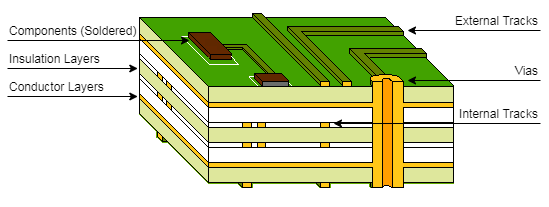
\includegraphics[width=0.85\textwidth]{figures/pcb_theory_example.png}
        \caption{Conceptual PCB board.}
        \label{fig:pcb_theory_example}
    \end{center}
\end{figure}


%1. Cubesat and Payloads standard
%\\2. Radiation issue overview
%\\3. SDRAMs operation and radiation
%\\4. FPGAs features and radiation
%\\5. PCB principles, guidelines and standards


\clearpage